\section{PLANTEAMIENTO DEL PROBLEMA}

\subsection{Descripción del Problema y Asimetría de Mercado}
En el mercado boliviano de bienes de consumo masivo y productos farmacéuticos coexiste una marcada fragmentación de precios. El consumidor promedio se enfrenta a variaciones sustanciales en el costo final de un mismo producto dependiendo de la cadena comercial, la ubicación geográfica de la sucursal o el canal de venta (físico o digital). En el rubro farmacéutico, esta asimetría adquiere especial gravedad: medicamentos esenciales como el \textit{Paracetamol 500 mg}, el \textit{Ibuprofeno 400 mg} o el \textit{Losartán 50 mg} pueden registrar diferenciales de precio superiores al 100\% entre cadenas competidoras o incluso entre presentaciones de marca e insumos genéricos. 

La falta de herramientas centralizadas y públicas que comparen estas variaciones en tiempo real genera ineficiencias en el gasto familiar e incrementa los costos de búsqueda para los ciudadanos, quienes deben visitar manualmente múltiples sucursales o navegar portales web desconectados entre sí.

\subsection{Vulnerabilidad de los Mecanismos de Extracción Tradicionales}
La recolección masiva de datos en la web moderna enfrenta obstáculos técnicos de alta complejidad. La mayoría de los supermercados y farmacias han adoptado esquemas de renderizado dinámico en el cliente y mecanismos de defensa automatizados contra bots. Como se ilustra en la Figura~\ref{fig:radware_challenge}, plataformas como Hipermaxi implementan capas de seguridad perimetral provistas por \textbf{Radware Bot Manager}, las cuales interceptan las conexiones automáticas y despliegan desafíos interactivos de tipo \textit{hCAPTCHA} cuando detectan firmas sintéticas o ausencia de interacción táctil o de puntero humano.

\begin{figure}[htbp]
    \centering
    \caption{Desafío de Verificación Humana de Radware Bot Manager en Plataforma Hipermaxi}
    \label{fig:radware_challenge}
    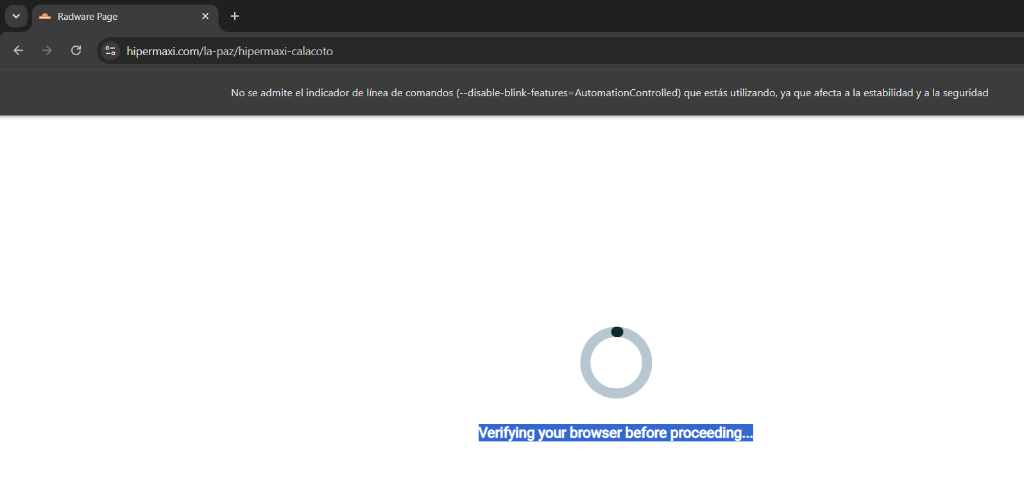
\includegraphics[width=0.85\linewidth]{figuras/radware_bot_manager_challenge.png}
    \figurenote{Pantalla de intercepción de tráfico emitida por Radware Bot Manager en el portal de Hipermaxi Bolivia. Demuestra el bloqueo inmediato de scrapers no instrumentados y justifica la necesidad de utilizar navegadores reales con perfiles persistentes y emulación de interacción humana.}
\end{figure}

Cuando los bots automatizados persisten en peticiones recurrentes sin almacenar estado o fallan al responder los desafíos criptográficos iniciales de JavaScript, Radware escala la protección hacia un segundo nivel más restrictivo: la pantalla de detección de anomalías con reto interactivo \textit{hCaptcha} (Figura~\ref{fig:radware_captcha}).

\begin{figure}[htbp]
    \centering
    \caption{Intercepción Activa de Radware Bot Manager con Desafío hCaptcha ante Anomalías}
    \label{fig:radware_captcha}
    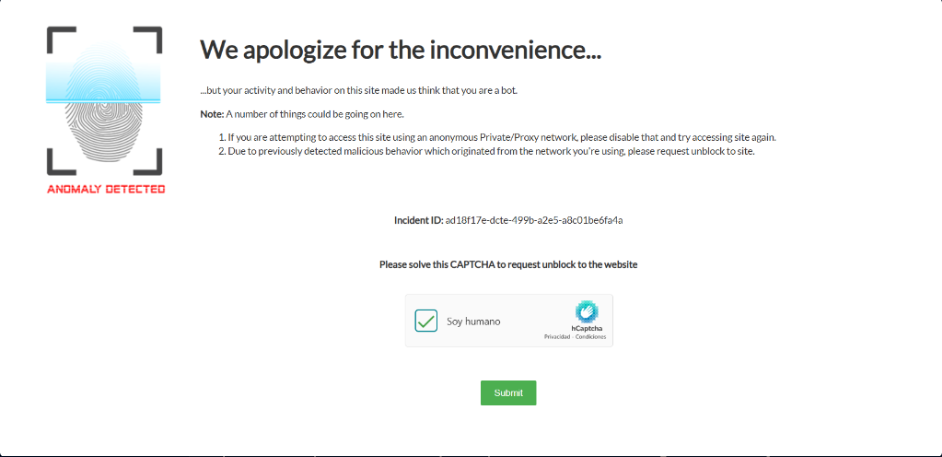
\includegraphics[width=0.85\linewidth]{figuras/imgADVERTENCIA1.png}
    \figurenote{Respuesta perimetral de Radware Bot Manager al detectar anomalías en la firma de navegación o patrones automatizados. Demuestra la escalada hacia retos interactivos de verificación humana (\textit{hCaptcha}) que invalidan los scrapers basados en peticiones HTTP estáticas.}
\end{figure}

A este blindaje perimetral se añade la complejidad del renderizado dinámico en el navegador del cliente (\textit{Single Page Application}). Plataformas como Hipermaxi no estructuran sus catálogos mediante páginas numeradas estáticas, sino a través de desplazamiento vertical asíncrono (\textit{infinite scrolling}). Al alcanzar el límite inferior de la vista, la aplicación inyecta componentes reactivos de carga con animaciones giratorias (Figura~\ref{fig:hipermaxi_spinner}), exigiendo sincronización precisa para no truncar la recolección de productos.

\begin{figure}[htbp]
    \centering
    \caption{Indicador Asíncrono de Carga en Catálogo SPA de Hipermaxi Bolivia}
    \label{fig:hipermaxi_spinner}
    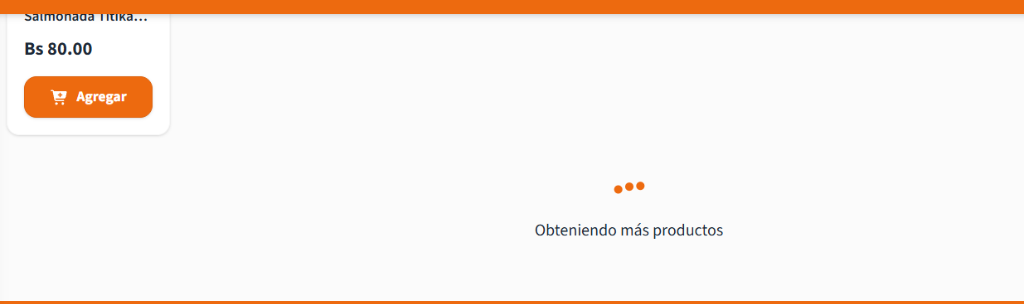
\includegraphics[width=0.82\linewidth]{figuras/hipermaxi_scroll_infinito_spinner.png}
    \figurenote{Captura del DOM dinámico en Hipermaxi durante el desplazamiento vertical. El elemento reactivo \texttt{span:has-text("Obteniendo más productos")} con animación giratoria (\textit{spinner}) exige algoritmos de sincronización basados en eventos de red y mutaciones de interfaz.}
\end{figure}

Los métodos convencionales de web scraping, basados en clientes HTTP sin motor de renderizado de JavaScript o en instancias efímeras de navegadores sin almacenamiento de estado, fracasan sistemáticamente ante estas defensas. Esto provoca la interrupción de los flujos de ingesta y la generación de conjuntos de datos incompletos o corruptos.

\subsection{Inadecuación de Modelos de Base de Datos Convencionales}
A nivel de persistencia de datos, el almacenamiento ingenuo de observaciones de precios en tablas transaccionales únicas sin normalización ocasiona redundancia masiva de atributos inmutables (nombres de producto, marcas, categorías, enlaces a imágenes). Al mismo tiempo, las operaciones de actualización masiva (\textit{UPSERT}) generan bloqueos a nivel de página o tabla (\textit{table locks}), degradando severamente el rendimiento de las consultas analíticas del usuario final. Para monitorear la inflación local y la volatilidad de precios, se requiere un modelo de series temporales capaz de computar instantáneamente la variación monetaria ($\Delta\text{Bs} = P_t - P_{t-1}$) y la tasa porcentual ($\Delta\%$), preservando el rendimiento mediante particionamiento temporal y disparadores reactivos desacoplados.

\subsection{Pregunta Formal de Investigación e Hipótesis}

\begin{interpretacionbox}
\textbf{Pregunta de Investigación:}  
¿De qué manera es posible estructurar un sistema integral de minería web multidimensional (contenido, estructura y uso) que supere de forma automatizada y resiliente las defensas perimetrales WAF en plataformas retail bolivianas, almacene de manera eficiente series de tiempo de precios en una base de datos serverless normalizada y provea a la ciudadanía herramientas interactivas de comparación de ahorro y geolocalización de servicios de salud?
\end{interpretacionbox}

\vspace{0.3cm}
\noindent \textbf{Hipótesis Tecnológica:}  
El diseño de agentes de extracción instrumentados con Playwright sobre contextos persistentes, coordinados con una arquitectura relacional en Neon Serverless PostgreSQL mediante triggers reactivos PL/pgSQL y particionamiento declarativo mensual, permite recolectar y procesar con una tasa de éxito superior al 98\% los catálogos en línea del eje central, habilitando el cálculo en tiempo real de variaciones de precios y el modelado de redes de contratación pública para su acceso masivo vía Telegram y Next.js 14.
